\documentclass[../main]{subfiles}

\begin{document}
\section{Hoja de ruta}

\subsection{Programación de aplicación}

\subsubsection{Recursos a usar}

\begin{itemize}
	\item Kotlin: Lenguaje principal de desarrollo
	      \url{https://developer.android.com/studio?hl=es-419}
	\item Firebase Authentication: Para la autenticación de los usuarios
	      \url{https://firebase.google.com/?hl=es-419}
	\item AndroidPlot: Biblioteca para la visualización de gráficos
	      \url{https://github.com/halfhp/androidplot/blob/master/docs/quickstart.md }
	\item Conexión WiFi (ESP32)
\end{itemize}

\subsubsection{Registro e Inicio de Sesión}

\begin{itemize}
	\item Registro de Usuario
	      El usuario podrá crear una cuenta proporcionando un correo electrónico
	      válido y configurando una contraseña segura.
	\item Inicio de Sesión
	      Los usuarios que ya se hayan registrado podrán iniciar sesión ingresando
	      su correo electrónico y contraseña. El uso de Firebase Authentication
	      se usará para el proceso de autenticación.
\end{itemize}

\begin{figure}[H]
	\centering
	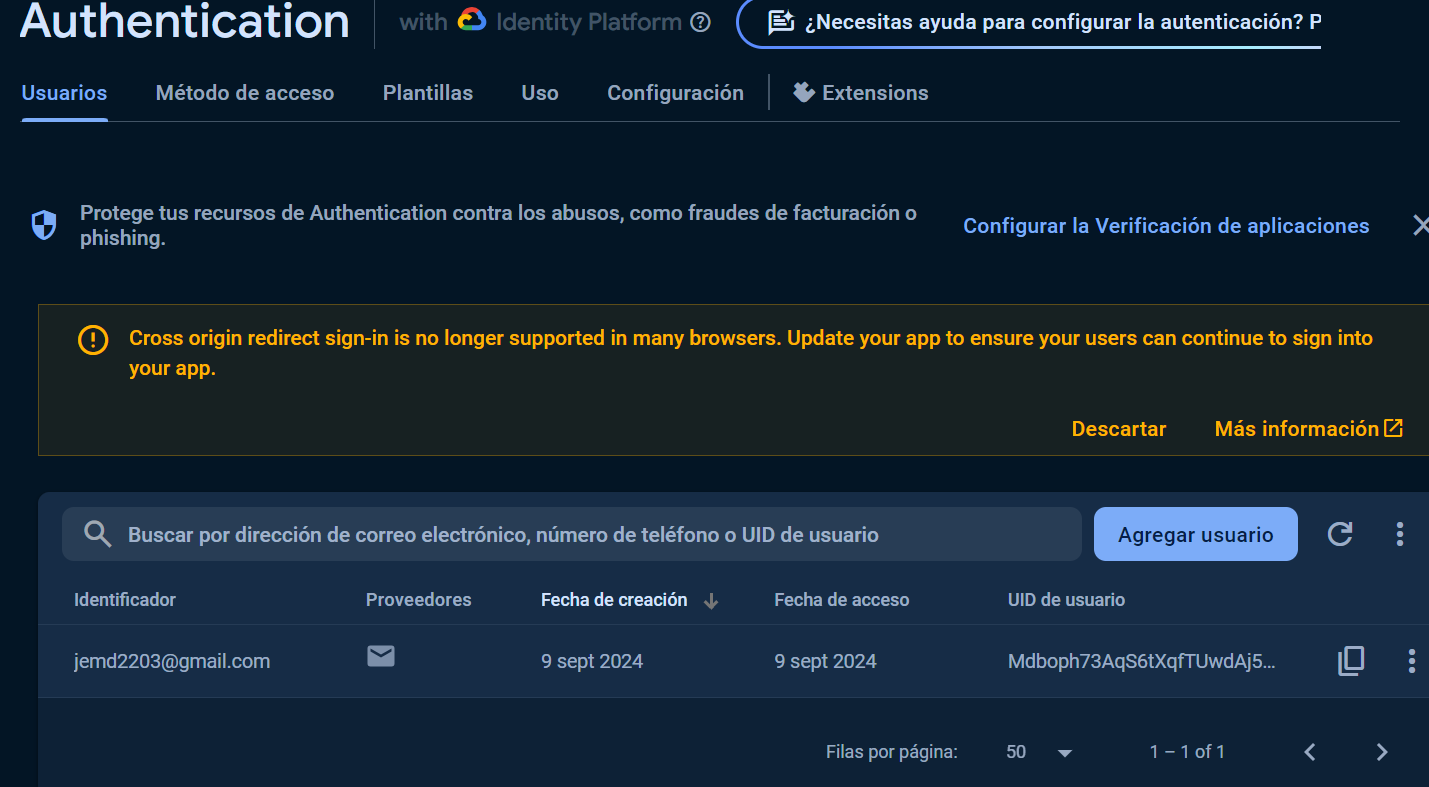
\includegraphics[width=15cm]{res/AutenticacionFireBase.png}
	\caption{Usuario registrado en Firebase}
	\label{FiguraDeAutenticacion}
\end{figure}

\subsubsection{Conectar Dispositivo}

\begin{itemize}
	\item Conexión a través de WiFi:
	      La conexión entre la aplicación y el dispositivo se llevará a cabo a
	      través de la red WiFi, permitiendo la comunicación en tiempo real.
	\item Interfaz de Conexión:
	      Habrá una pantalla específica donde el usuario podrá buscar y seleccionar
	      el dispositivo ESP32 dentro de la red disponible.
	      Una vez conectado, la aplicación podrá recibir los datos de los sensores
	      y mostrarlos de manera continua.

\end{itemize}

\subsubsection{Visualización de Datos y Gráficos}

\begin{itemize}
	\item Parámetros Ambientales:
	      Los valores de temperatura, humedad, presión y concentración de \ce{CO2} se
	      mostrarán de forma intuitiva en la pantalla principal de la aplicación
	      para monitorear constantemente las condiciones del invernadero.
	\item Generación de Gráficos:
	      La aplicación permitirá también la visualización gráfica de los datos
	      históricos. Para implementar esta funcionalidad, se usará la biblioteca
	      AndroidPlot que facilita la creación de gráficos de líneas, gráficos de
	      barras y otras representaciones visuales.
	\item Datos Históricos:
	      Los usuarios podrán acceder a un historial de las condiciones ambientales
	      registradas, lo cual será útil para la toma de decisiones relacionadas
	      con el cultivo.
\end{itemize}

\begin{figure}[H]
	\centering
	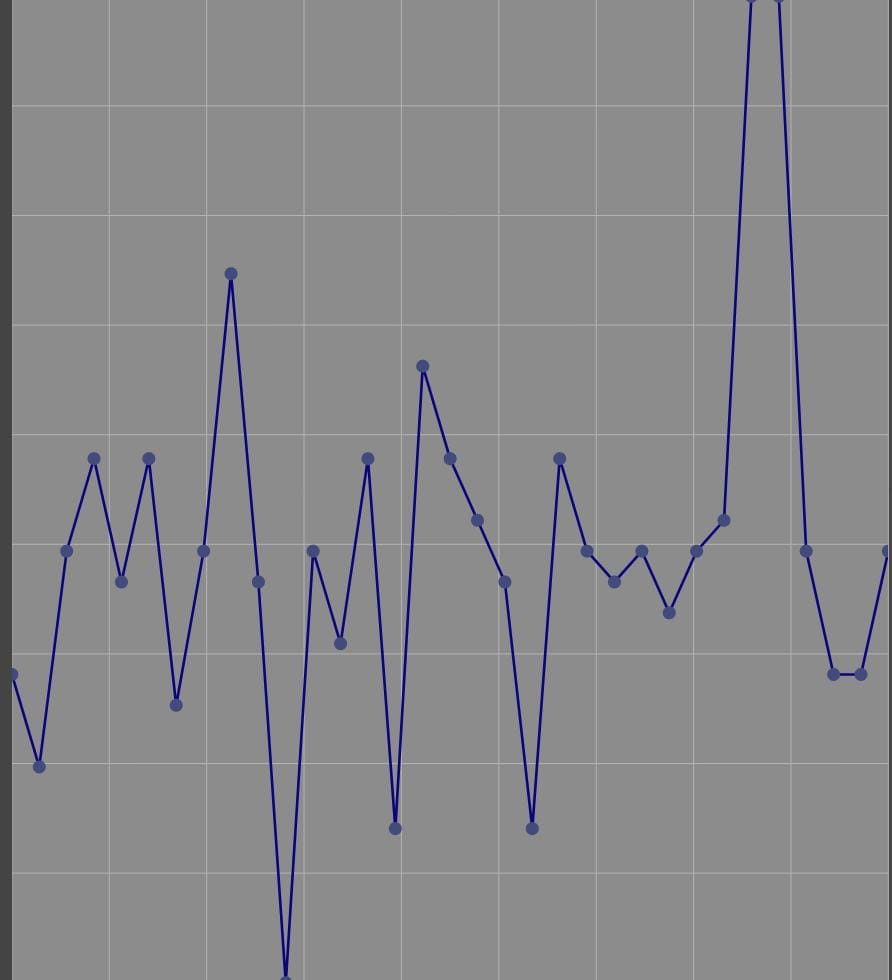
\includegraphics[width=10cm]{res/GráficosParaAplicación.jpeg}
	\caption{Gráficos generado por biblioteca}
	\label{FiguraDeGráficos}
\end{figure}

\subsubsection{ Diseño de la Interfaz de Usuario}

\begin{itemize}
	\item Menú de Navegación:
	      La aplicación tendrá un menú de navegación que permitirá al usuario
	      acceder fácilmente a las diferentes secciones: registro/inicio de
	      sesión, conexión de dispositivo, y visualización de datos.
	\item Pantalla Principal:
	      Una vez conectado el dispositivo, la pantalla principal mostrará
	      los valores actuales de temperatura, humedad, presión y \ce{CO2}.
	\item Pantalla de Gráficos:
	      Incluirá un apartado para la visualización de gráficos, donde el usuario
	      podrá seleccionar el parámetro que desea visualizar y el intervalo de
	      tiempo.
\end{itemize}

\subsubsection{Notificaciones y Alertas}

Se integrarán notificaciones para alertar al usuario cuando algún parámetro
ambiental esté fuera de los rangos definidos como óptimos.
Esto permitirá al usuario tomar medidas correctivas según lo que observe como
necesario para el mantenimiento del invernadero.

\subsection{Configuración de Hardware}

\subsubsection{Recursos a usar}

\begin{itemize}
	\item ESP32: Controlador principal con conectividad WiFi.
	\item Sensor BME280: Sensor para medir temperatura, humedad y presión.
	\item Sensor MQ135: Sensor para la detección de la concentración de CO2 en el aire.
	\item Sensor de Humedad de Suelo: Sensor analógico para medir el nivel de humedad del suelo.
	\item Protoboard y Jumpers: Para facilitar las conexiones de prueba.
	\item Fuente de Alimentación: Batería o adaptador USB de 5V.
	\item Cables Dupont: Para realizar las conexiones entre los sensores y el ESP32.
\end{itemize}

\subsubsection{ Diagrama de Conexiones}

\begin{itemize}
	\item ESP32: Este será el controlador principal y estará encargado de leer los datos de cada sensor.
	\item BME280: Este sensor utiliza la comunicación I2C para conectarse con el ESP32. Las conexiones necesarias son:
	      \begin{enumerate}
		      \item VCC a 3.3V del ESP32.
		      \item GND a GND del ESP32.
		      \item SCL al pin D22 del ESP32.
		      \item SDA al pin D21 del ESP32.
	      \end{enumerate}
	\item MQ135: Para el sensor MQ135, se utilizará la salida analógica para la detección de CO2.
	      \begin{enumerate}
		      \item VCC a 5V del ESP32.
		      \item GND a GND del ESP32.
		      \item AOUT a un pin analógico del ESP32.
	      \end{enumerate}
	\item Sensor de Humedad de Suelo: El sensor de humedad de suelo puede ser analógico o digital. Se optará por la salida analógica para una medición más precisa.
	      \begin{enumerate}
		      \item VCC a 3.3V del ESP32.
		      \item GND a GND del ESP32.
		      \item AOUT a un pin analógico del ESP32.
	      \end{enumerate}
\end{itemize}

\subsubsection{Programación}

Antes de comenzar a programar tu ESP32, aseg\'urate de tener instalados los controladores y bibliotecas necesarias para trabajar en Arduino IDE.

\subsubsection{Soporte del ESP32 en Arduino IDE:}

Para poder programar en ESP32 con Arduino se necesita agregar un URL en el gestor de placas lo siguiente:
\url{https://dl.espressif.com/dl/package_esp32_index.json}

\begin{figure}[H]
	\centering
	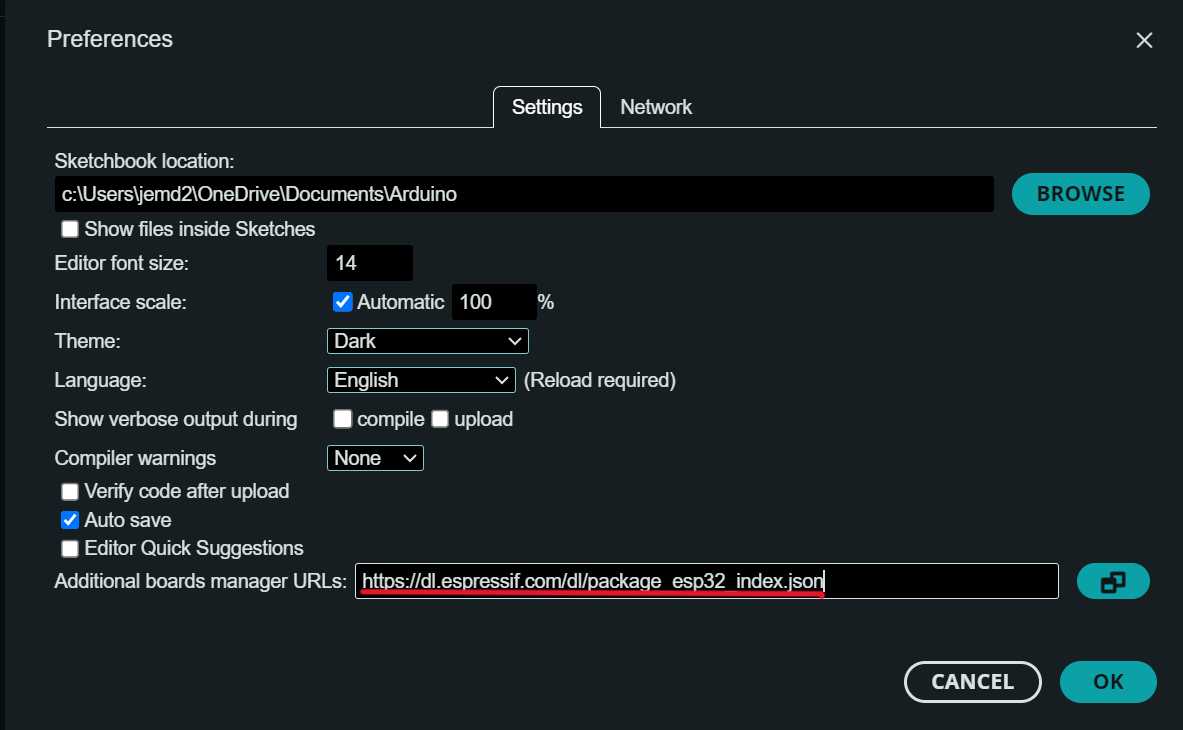
\includegraphics[width = 13cm]{res/configuracionParaEsp32.png}
\end{figure}

\subsubsection{Conexión con Firebase}

Para realizar una conexión a Firebase desde tu ESP32, necesitas la biblioteca Firebase ESP32 Client.
\end{document}
